\documentclass[aspectratio=169]{beamer}
% Shared preamble for ml/ slide decks.
% Each lecture .tex starts with:
%   \documentclass[aspectratio=169]{beamer}
%   % Shared preamble for ml/ slide decks.
% Each lecture .tex starts with:
%   \documentclass[aspectratio=169]{beamer}
%   % Shared preamble for ml/ slide decks.
% Each lecture .tex starts with:
%   \documentclass[aspectratio=169]{beamer}
%   \input{../preamble}
% Compile from inside the chapter folder so \input{../preamble} resolves.

\usetheme{default}
\usecolortheme{dove}

\setbeamertemplate{navigation symbols}{}
\setbeamertemplate{footline}{%
  \hfill{\large\insertframenumber\,/\,\inserttotalframenumber}\hspace{0.8em}\vspace{0.5em}%
}

% Project palette (existing, kept for backwards compatibility with deferred/*)
\definecolor{popblue}{RGB}{52, 101, 164}
\definecolor{sampred}{RGB}{204, 0, 0}
\definecolor{paramgreen}{RGB}{0, 140, 70}
\definecolor{warnred}{RGB}{180, 40, 40}
\definecolor{orange1}{RGB}{220, 120, 0}
\definecolor{violet1}{RGB}{120, 50, 160}
\definecolor{lightbg}{RGB}{245, 245, 250}

% Armenian flag palette (use these for any 3-color highlight; per CLAUDE.md).
% "Nice versions": slightly de-saturated from the official spec for slide use,
% so they don't burn out under projector colors. Originals kept as *_pure.
\definecolor{armred}{RGB}{200, 30, 40}      % nice red (official #D90012 muted)
\definecolor{armblue}{RGB}{30, 70, 160}     % nice blue (official #0033A0 muted)
\definecolor{armorange}{RGB}{230, 160, 30}  % nice orange (official #F2A800 muted)
\definecolor{armred_pure}{HTML}{D90012}     % official Armenian flag red
\definecolor{armblue_pure}{HTML}{0033A0}    % official Armenian flag blue
\definecolor{armorange_pure}{HTML}{F2A800}  % official Armenian flag orange

\setbeamercolor{frametitle}{fg=popblue}
\setbeamercolor{title}{fg=popblue}

\usepackage{pgfplots}
\usepackage{tikz}
\usetikzlibrary{shapes, arrows.meta, positioning, calc, decorations.pathreplacing, patterns, matrix}
\pgfplotsset{compat=1.18}
\usepackage{amsmath, amssymb, amsfonts}
\usepackage{bm}
\usepackage{dsfont}
\usepackage{array}
\usepackage{pifont}
\usepackage{colortbl}
\usepackage{fontenc}

% Callout boxes. Purely additive - existing decks are unaffected.
% Usage: \begin{tcolorbox}[colback=armblue!8, colframe=armblue, boxrule=0.6pt, arc=2pt,
%                          title=\textbf{Key idea}] ... \end{tcolorbox}
% Palette convention (ml/SLIDE_STYLE.md): armblue=key idea, armred=trap/warning,
% paramgreen=takeaway or "Next", armorange=watch-out.
\usepackage[most]{tcolorbox}

% Cleaner table rules (\toprule, \midrule, \bottomrule). Also purely additive.
\usepackage{booktabs}

% \cancel{...} for struck-through terms in derivations (added 2026-08-11 for the
% importance-sampling frame in ch11_rl, where the dynamics cancel). Purely additive.
\usepackage{cancel}

% Minimal ML notation macros (subset of slds-lmu latex-math/basic-ml.tex).
% Kept here so we don't have to inline-expand every \thetav, \xv, etc.
% when porting upstream slides.
\newcommand{\R}{\mathds{R}}
\newcommand{\N}{\mathds{N}}
\newcommand{\E}{\mathds{E}}
\newcommand{\Xspace}{\mathcal{X}}
\newcommand{\Yspace}{\mathcal{Y}}
\newcommand{\Hspace}{\mathcal{H}}
\newcommand{\D}{\mathcal{D}}
\newcommand{\Dtrain}{\mathcal{D}_{\text{train}}}
\newcommand{\Dtest}{\mathcal{D}_{\text{test}}}
\newcommand{\xv}{\mathbf{x}}
\newcommand{\yv}{\mathbf{y}}
\newcommand{\Xmat}{\mathbf{X}}
\newcommand{\id}{\mathbf{I}}
\newcommand{\thetav}{\bm{\theta}}
\newcommand{\thetah}{\hat{\bm{\theta}}}
\newcommand{\lamv}{\bm{\lambda}}
\newcommand{\fx}{f(\xv)}
\newcommand{\fxt}{f(\xv \,|\, \bm{\theta})}
\newcommand{\fxi}{f\!\left(\xv^{(i)}\right)}
\newcommand{\fh}{\hat{f}}
\newcommand{\fxh}{\hat{f}(\xv)}
\newcommand{\yh}{\hat{y}}
\newcommand{\yih}{\hat{y}^{(i)}}
% \xi clashes with the Greek letter \xi; write \xv^{(i)} inline instead.
\newcommand{\yi}[1][i]{y^{(#1)}}
\newcommand{\xyi}[1][i]{\left(\xv^{(#1)},\, y^{(#1)}\right)}
\newcommand{\thx}{\bm{\theta}^\top \xv}
\newcommand{\sumin}{\sum_{i=1}^{n}}
\newcommand{\sumjp}{\sum_{j=1}^{p}}
\newcommand{\Lxy}{L\!\left(y, \fx\right)}
\newcommand{\Lxyi}{L\!\left(\yi, \fxi\right)}
\newcommand{\risk}{\mathcal{R}}
\newcommand{\riske}{\mathcal{R}_{\text{emp}}}
\newcommand{\risket}{\mathcal{R}_{\text{emp}}(\bm{\theta})}
\newcommand{\riskt}{\mathcal{R}(\bm{\theta})}
\newcommand{\riskr}{\mathcal{R}_{\text{reg}}}
\newcommand{\argmin}{\mathop{\mathrm{arg\,min}}}
\newcommand{\argmax}{\mathop{\mathrm{arg\,max}}}
\newcommand{\eps}{\varepsilon}

% Compile from inside the chapter folder so % Shared preamble for ml/ slide decks.
% Each lecture .tex starts with:
%   \documentclass[aspectratio=169]{beamer}
%   \input{../preamble}
% Compile from inside the chapter folder so \input{../preamble} resolves.

\usetheme{default}
\usecolortheme{dove}

\setbeamertemplate{navigation symbols}{}
\setbeamertemplate{footline}{%
  \hfill{\large\insertframenumber\,/\,\inserttotalframenumber}\hspace{0.8em}\vspace{0.5em}%
}

% Project palette (existing, kept for backwards compatibility with deferred/*)
\definecolor{popblue}{RGB}{52, 101, 164}
\definecolor{sampred}{RGB}{204, 0, 0}
\definecolor{paramgreen}{RGB}{0, 140, 70}
\definecolor{warnred}{RGB}{180, 40, 40}
\definecolor{orange1}{RGB}{220, 120, 0}
\definecolor{violet1}{RGB}{120, 50, 160}
\definecolor{lightbg}{RGB}{245, 245, 250}

% Armenian flag palette (use these for any 3-color highlight; per CLAUDE.md).
% "Nice versions": slightly de-saturated from the official spec for slide use,
% so they don't burn out under projector colors. Originals kept as *_pure.
\definecolor{armred}{RGB}{200, 30, 40}      % nice red (official #D90012 muted)
\definecolor{armblue}{RGB}{30, 70, 160}     % nice blue (official #0033A0 muted)
\definecolor{armorange}{RGB}{230, 160, 30}  % nice orange (official #F2A800 muted)
\definecolor{armred_pure}{HTML}{D90012}     % official Armenian flag red
\definecolor{armblue_pure}{HTML}{0033A0}    % official Armenian flag blue
\definecolor{armorange_pure}{HTML}{F2A800}  % official Armenian flag orange

\setbeamercolor{frametitle}{fg=popblue}
\setbeamercolor{title}{fg=popblue}

\usepackage{pgfplots}
\usepackage{tikz}
\usetikzlibrary{shapes, arrows.meta, positioning, calc, decorations.pathreplacing, patterns, matrix}
\pgfplotsset{compat=1.18}
\usepackage{amsmath, amssymb, amsfonts}
\usepackage{bm}
\usepackage{dsfont}
\usepackage{array}
\usepackage{pifont}
\usepackage{colortbl}
\usepackage{fontenc}

% Callout boxes. Purely additive - existing decks are unaffected.
% Usage: \begin{tcolorbox}[colback=armblue!8, colframe=armblue, boxrule=0.6pt, arc=2pt,
%                          title=\textbf{Key idea}] ... \end{tcolorbox}
% Palette convention (ml/SLIDE_STYLE.md): armblue=key idea, armred=trap/warning,
% paramgreen=takeaway or "Next", armorange=watch-out.
\usepackage[most]{tcolorbox}

% Cleaner table rules (\toprule, \midrule, \bottomrule). Also purely additive.
\usepackage{booktabs}

% \cancel{...} for struck-through terms in derivations (added 2026-08-11 for the
% importance-sampling frame in ch11_rl, where the dynamics cancel). Purely additive.
\usepackage{cancel}

% Minimal ML notation macros (subset of slds-lmu latex-math/basic-ml.tex).
% Kept here so we don't have to inline-expand every \thetav, \xv, etc.
% when porting upstream slides.
\newcommand{\R}{\mathds{R}}
\newcommand{\N}{\mathds{N}}
\newcommand{\E}{\mathds{E}}
\newcommand{\Xspace}{\mathcal{X}}
\newcommand{\Yspace}{\mathcal{Y}}
\newcommand{\Hspace}{\mathcal{H}}
\newcommand{\D}{\mathcal{D}}
\newcommand{\Dtrain}{\mathcal{D}_{\text{train}}}
\newcommand{\Dtest}{\mathcal{D}_{\text{test}}}
\newcommand{\xv}{\mathbf{x}}
\newcommand{\yv}{\mathbf{y}}
\newcommand{\Xmat}{\mathbf{X}}
\newcommand{\id}{\mathbf{I}}
\newcommand{\thetav}{\bm{\theta}}
\newcommand{\thetah}{\hat{\bm{\theta}}}
\newcommand{\lamv}{\bm{\lambda}}
\newcommand{\fx}{f(\xv)}
\newcommand{\fxt}{f(\xv \,|\, \bm{\theta})}
\newcommand{\fxi}{f\!\left(\xv^{(i)}\right)}
\newcommand{\fh}{\hat{f}}
\newcommand{\fxh}{\hat{f}(\xv)}
\newcommand{\yh}{\hat{y}}
\newcommand{\yih}{\hat{y}^{(i)}}
% \xi clashes with the Greek letter \xi; write \xv^{(i)} inline instead.
\newcommand{\yi}[1][i]{y^{(#1)}}
\newcommand{\xyi}[1][i]{\left(\xv^{(#1)},\, y^{(#1)}\right)}
\newcommand{\thx}{\bm{\theta}^\top \xv}
\newcommand{\sumin}{\sum_{i=1}^{n}}
\newcommand{\sumjp}{\sum_{j=1}^{p}}
\newcommand{\Lxy}{L\!\left(y, \fx\right)}
\newcommand{\Lxyi}{L\!\left(\yi, \fxi\right)}
\newcommand{\risk}{\mathcal{R}}
\newcommand{\riske}{\mathcal{R}_{\text{emp}}}
\newcommand{\risket}{\mathcal{R}_{\text{emp}}(\bm{\theta})}
\newcommand{\riskt}{\mathcal{R}(\bm{\theta})}
\newcommand{\riskr}{\mathcal{R}_{\text{reg}}}
\newcommand{\argmin}{\mathop{\mathrm{arg\,min}}}
\newcommand{\argmax}{\mathop{\mathrm{arg\,max}}}
\newcommand{\eps}{\varepsilon}
 resolves.

\usetheme{default}
\usecolortheme{dove}

\setbeamertemplate{navigation symbols}{}
\setbeamertemplate{footline}{%
  \hfill{\large\insertframenumber\,/\,\inserttotalframenumber}\hspace{0.8em}\vspace{0.5em}%
}

% Project palette (existing, kept for backwards compatibility with deferred/*)
\definecolor{popblue}{RGB}{52, 101, 164}
\definecolor{sampred}{RGB}{204, 0, 0}
\definecolor{paramgreen}{RGB}{0, 140, 70}
\definecolor{warnred}{RGB}{180, 40, 40}
\definecolor{orange1}{RGB}{220, 120, 0}
\definecolor{violet1}{RGB}{120, 50, 160}
\definecolor{lightbg}{RGB}{245, 245, 250}

% Armenian flag palette (use these for any 3-color highlight; per CLAUDE.md).
% "Nice versions": slightly de-saturated from the official spec for slide use,
% so they don't burn out under projector colors. Originals kept as *_pure.
\definecolor{armred}{RGB}{200, 30, 40}      % nice red (official #D90012 muted)
\definecolor{armblue}{RGB}{30, 70, 160}     % nice blue (official #0033A0 muted)
\definecolor{armorange}{RGB}{230, 160, 30}  % nice orange (official #F2A800 muted)
\definecolor{armred_pure}{HTML}{D90012}     % official Armenian flag red
\definecolor{armblue_pure}{HTML}{0033A0}    % official Armenian flag blue
\definecolor{armorange_pure}{HTML}{F2A800}  % official Armenian flag orange

\setbeamercolor{frametitle}{fg=popblue}
\setbeamercolor{title}{fg=popblue}

\usepackage{pgfplots}
\usepackage{tikz}
\usetikzlibrary{shapes, arrows.meta, positioning, calc, decorations.pathreplacing, patterns, matrix}
\pgfplotsset{compat=1.18}
\usepackage{amsmath, amssymb, amsfonts}
\usepackage{bm}
\usepackage{dsfont}
\usepackage{array}
\usepackage{pifont}
\usepackage{colortbl}
\usepackage{fontenc}

% Callout boxes. Purely additive - existing decks are unaffected.
% Usage: \begin{tcolorbox}[colback=armblue!8, colframe=armblue, boxrule=0.6pt, arc=2pt,
%                          title=\textbf{Key idea}] ... \end{tcolorbox}
% Palette convention (ml/SLIDE_STYLE.md): armblue=key idea, armred=trap/warning,
% paramgreen=takeaway or "Next", armorange=watch-out.
\usepackage[most]{tcolorbox}

% Cleaner table rules (\toprule, \midrule, \bottomrule). Also purely additive.
\usepackage{booktabs}

% \cancel{...} for struck-through terms in derivations (added 2026-08-11 for the
% importance-sampling frame in ch11_rl, where the dynamics cancel). Purely additive.
\usepackage{cancel}

% Minimal ML notation macros (subset of slds-lmu latex-math/basic-ml.tex).
% Kept here so we don't have to inline-expand every \thetav, \xv, etc.
% when porting upstream slides.
\newcommand{\R}{\mathds{R}}
\newcommand{\N}{\mathds{N}}
\newcommand{\E}{\mathds{E}}
\newcommand{\Xspace}{\mathcal{X}}
\newcommand{\Yspace}{\mathcal{Y}}
\newcommand{\Hspace}{\mathcal{H}}
\newcommand{\D}{\mathcal{D}}
\newcommand{\Dtrain}{\mathcal{D}_{\text{train}}}
\newcommand{\Dtest}{\mathcal{D}_{\text{test}}}
\newcommand{\xv}{\mathbf{x}}
\newcommand{\yv}{\mathbf{y}}
\newcommand{\Xmat}{\mathbf{X}}
\newcommand{\id}{\mathbf{I}}
\newcommand{\thetav}{\bm{\theta}}
\newcommand{\thetah}{\hat{\bm{\theta}}}
\newcommand{\lamv}{\bm{\lambda}}
\newcommand{\fx}{f(\xv)}
\newcommand{\fxt}{f(\xv \,|\, \bm{\theta})}
\newcommand{\fxi}{f\!\left(\xv^{(i)}\right)}
\newcommand{\fh}{\hat{f}}
\newcommand{\fxh}{\hat{f}(\xv)}
\newcommand{\yh}{\hat{y}}
\newcommand{\yih}{\hat{y}^{(i)}}
% \xi clashes with the Greek letter \xi; write \xv^{(i)} inline instead.
\newcommand{\yi}[1][i]{y^{(#1)}}
\newcommand{\xyi}[1][i]{\left(\xv^{(#1)},\, y^{(#1)}\right)}
\newcommand{\thx}{\bm{\theta}^\top \xv}
\newcommand{\sumin}{\sum_{i=1}^{n}}
\newcommand{\sumjp}{\sum_{j=1}^{p}}
\newcommand{\Lxy}{L\!\left(y, \fx\right)}
\newcommand{\Lxyi}{L\!\left(\yi, \fxi\right)}
\newcommand{\risk}{\mathcal{R}}
\newcommand{\riske}{\mathcal{R}_{\text{emp}}}
\newcommand{\risket}{\mathcal{R}_{\text{emp}}(\bm{\theta})}
\newcommand{\riskt}{\mathcal{R}(\bm{\theta})}
\newcommand{\riskr}{\mathcal{R}_{\text{reg}}}
\newcommand{\argmin}{\mathop{\mathrm{arg\,min}}}
\newcommand{\argmax}{\mathop{\mathrm{arg\,max}}}
\newcommand{\eps}{\varepsilon}

% Compile from inside the chapter folder so % Shared preamble for ml/ slide decks.
% Each lecture .tex starts with:
%   \documentclass[aspectratio=169]{beamer}
%   % Shared preamble for ml/ slide decks.
% Each lecture .tex starts with:
%   \documentclass[aspectratio=169]{beamer}
%   \input{../preamble}
% Compile from inside the chapter folder so \input{../preamble} resolves.

\usetheme{default}
\usecolortheme{dove}

\setbeamertemplate{navigation symbols}{}
\setbeamertemplate{footline}{%
  \hfill{\large\insertframenumber\,/\,\inserttotalframenumber}\hspace{0.8em}\vspace{0.5em}%
}

% Project palette (existing, kept for backwards compatibility with deferred/*)
\definecolor{popblue}{RGB}{52, 101, 164}
\definecolor{sampred}{RGB}{204, 0, 0}
\definecolor{paramgreen}{RGB}{0, 140, 70}
\definecolor{warnred}{RGB}{180, 40, 40}
\definecolor{orange1}{RGB}{220, 120, 0}
\definecolor{violet1}{RGB}{120, 50, 160}
\definecolor{lightbg}{RGB}{245, 245, 250}

% Armenian flag palette (use these for any 3-color highlight; per CLAUDE.md).
% "Nice versions": slightly de-saturated from the official spec for slide use,
% so they don't burn out under projector colors. Originals kept as *_pure.
\definecolor{armred}{RGB}{200, 30, 40}      % nice red (official #D90012 muted)
\definecolor{armblue}{RGB}{30, 70, 160}     % nice blue (official #0033A0 muted)
\definecolor{armorange}{RGB}{230, 160, 30}  % nice orange (official #F2A800 muted)
\definecolor{armred_pure}{HTML}{D90012}     % official Armenian flag red
\definecolor{armblue_pure}{HTML}{0033A0}    % official Armenian flag blue
\definecolor{armorange_pure}{HTML}{F2A800}  % official Armenian flag orange

\setbeamercolor{frametitle}{fg=popblue}
\setbeamercolor{title}{fg=popblue}

\usepackage{pgfplots}
\usepackage{tikz}
\usetikzlibrary{shapes, arrows.meta, positioning, calc, decorations.pathreplacing, patterns, matrix}
\pgfplotsset{compat=1.18}
\usepackage{amsmath, amssymb, amsfonts}
\usepackage{bm}
\usepackage{dsfont}
\usepackage{array}
\usepackage{pifont}
\usepackage{colortbl}
\usepackage{fontenc}

% Callout boxes. Purely additive - existing decks are unaffected.
% Usage: \begin{tcolorbox}[colback=armblue!8, colframe=armblue, boxrule=0.6pt, arc=2pt,
%                          title=\textbf{Key idea}] ... \end{tcolorbox}
% Palette convention (ml/SLIDE_STYLE.md): armblue=key idea, armred=trap/warning,
% paramgreen=takeaway or "Next", armorange=watch-out.
\usepackage[most]{tcolorbox}

% Cleaner table rules (\toprule, \midrule, \bottomrule). Also purely additive.
\usepackage{booktabs}

% \cancel{...} for struck-through terms in derivations (added 2026-08-11 for the
% importance-sampling frame in ch11_rl, where the dynamics cancel). Purely additive.
\usepackage{cancel}

% Minimal ML notation macros (subset of slds-lmu latex-math/basic-ml.tex).
% Kept here so we don't have to inline-expand every \thetav, \xv, etc.
% when porting upstream slides.
\newcommand{\R}{\mathds{R}}
\newcommand{\N}{\mathds{N}}
\newcommand{\E}{\mathds{E}}
\newcommand{\Xspace}{\mathcal{X}}
\newcommand{\Yspace}{\mathcal{Y}}
\newcommand{\Hspace}{\mathcal{H}}
\newcommand{\D}{\mathcal{D}}
\newcommand{\Dtrain}{\mathcal{D}_{\text{train}}}
\newcommand{\Dtest}{\mathcal{D}_{\text{test}}}
\newcommand{\xv}{\mathbf{x}}
\newcommand{\yv}{\mathbf{y}}
\newcommand{\Xmat}{\mathbf{X}}
\newcommand{\id}{\mathbf{I}}
\newcommand{\thetav}{\bm{\theta}}
\newcommand{\thetah}{\hat{\bm{\theta}}}
\newcommand{\lamv}{\bm{\lambda}}
\newcommand{\fx}{f(\xv)}
\newcommand{\fxt}{f(\xv \,|\, \bm{\theta})}
\newcommand{\fxi}{f\!\left(\xv^{(i)}\right)}
\newcommand{\fh}{\hat{f}}
\newcommand{\fxh}{\hat{f}(\xv)}
\newcommand{\yh}{\hat{y}}
\newcommand{\yih}{\hat{y}^{(i)}}
% \xi clashes with the Greek letter \xi; write \xv^{(i)} inline instead.
\newcommand{\yi}[1][i]{y^{(#1)}}
\newcommand{\xyi}[1][i]{\left(\xv^{(#1)},\, y^{(#1)}\right)}
\newcommand{\thx}{\bm{\theta}^\top \xv}
\newcommand{\sumin}{\sum_{i=1}^{n}}
\newcommand{\sumjp}{\sum_{j=1}^{p}}
\newcommand{\Lxy}{L\!\left(y, \fx\right)}
\newcommand{\Lxyi}{L\!\left(\yi, \fxi\right)}
\newcommand{\risk}{\mathcal{R}}
\newcommand{\riske}{\mathcal{R}_{\text{emp}}}
\newcommand{\risket}{\mathcal{R}_{\text{emp}}(\bm{\theta})}
\newcommand{\riskt}{\mathcal{R}(\bm{\theta})}
\newcommand{\riskr}{\mathcal{R}_{\text{reg}}}
\newcommand{\argmin}{\mathop{\mathrm{arg\,min}}}
\newcommand{\argmax}{\mathop{\mathrm{arg\,max}}}
\newcommand{\eps}{\varepsilon}

% Compile from inside the chapter folder so % Shared preamble for ml/ slide decks.
% Each lecture .tex starts with:
%   \documentclass[aspectratio=169]{beamer}
%   \input{../preamble}
% Compile from inside the chapter folder so \input{../preamble} resolves.

\usetheme{default}
\usecolortheme{dove}

\setbeamertemplate{navigation symbols}{}
\setbeamertemplate{footline}{%
  \hfill{\large\insertframenumber\,/\,\inserttotalframenumber}\hspace{0.8em}\vspace{0.5em}%
}

% Project palette (existing, kept for backwards compatibility with deferred/*)
\definecolor{popblue}{RGB}{52, 101, 164}
\definecolor{sampred}{RGB}{204, 0, 0}
\definecolor{paramgreen}{RGB}{0, 140, 70}
\definecolor{warnred}{RGB}{180, 40, 40}
\definecolor{orange1}{RGB}{220, 120, 0}
\definecolor{violet1}{RGB}{120, 50, 160}
\definecolor{lightbg}{RGB}{245, 245, 250}

% Armenian flag palette (use these for any 3-color highlight; per CLAUDE.md).
% "Nice versions": slightly de-saturated from the official spec for slide use,
% so they don't burn out under projector colors. Originals kept as *_pure.
\definecolor{armred}{RGB}{200, 30, 40}      % nice red (official #D90012 muted)
\definecolor{armblue}{RGB}{30, 70, 160}     % nice blue (official #0033A0 muted)
\definecolor{armorange}{RGB}{230, 160, 30}  % nice orange (official #F2A800 muted)
\definecolor{armred_pure}{HTML}{D90012}     % official Armenian flag red
\definecolor{armblue_pure}{HTML}{0033A0}    % official Armenian flag blue
\definecolor{armorange_pure}{HTML}{F2A800}  % official Armenian flag orange

\setbeamercolor{frametitle}{fg=popblue}
\setbeamercolor{title}{fg=popblue}

\usepackage{pgfplots}
\usepackage{tikz}
\usetikzlibrary{shapes, arrows.meta, positioning, calc, decorations.pathreplacing, patterns, matrix}
\pgfplotsset{compat=1.18}
\usepackage{amsmath, amssymb, amsfonts}
\usepackage{bm}
\usepackage{dsfont}
\usepackage{array}
\usepackage{pifont}
\usepackage{colortbl}
\usepackage{fontenc}

% Callout boxes. Purely additive - existing decks are unaffected.
% Usage: \begin{tcolorbox}[colback=armblue!8, colframe=armblue, boxrule=0.6pt, arc=2pt,
%                          title=\textbf{Key idea}] ... \end{tcolorbox}
% Palette convention (ml/SLIDE_STYLE.md): armblue=key idea, armred=trap/warning,
% paramgreen=takeaway or "Next", armorange=watch-out.
\usepackage[most]{tcolorbox}

% Cleaner table rules (\toprule, \midrule, \bottomrule). Also purely additive.
\usepackage{booktabs}

% \cancel{...} for struck-through terms in derivations (added 2026-08-11 for the
% importance-sampling frame in ch11_rl, where the dynamics cancel). Purely additive.
\usepackage{cancel}

% Minimal ML notation macros (subset of slds-lmu latex-math/basic-ml.tex).
% Kept here so we don't have to inline-expand every \thetav, \xv, etc.
% when porting upstream slides.
\newcommand{\R}{\mathds{R}}
\newcommand{\N}{\mathds{N}}
\newcommand{\E}{\mathds{E}}
\newcommand{\Xspace}{\mathcal{X}}
\newcommand{\Yspace}{\mathcal{Y}}
\newcommand{\Hspace}{\mathcal{H}}
\newcommand{\D}{\mathcal{D}}
\newcommand{\Dtrain}{\mathcal{D}_{\text{train}}}
\newcommand{\Dtest}{\mathcal{D}_{\text{test}}}
\newcommand{\xv}{\mathbf{x}}
\newcommand{\yv}{\mathbf{y}}
\newcommand{\Xmat}{\mathbf{X}}
\newcommand{\id}{\mathbf{I}}
\newcommand{\thetav}{\bm{\theta}}
\newcommand{\thetah}{\hat{\bm{\theta}}}
\newcommand{\lamv}{\bm{\lambda}}
\newcommand{\fx}{f(\xv)}
\newcommand{\fxt}{f(\xv \,|\, \bm{\theta})}
\newcommand{\fxi}{f\!\left(\xv^{(i)}\right)}
\newcommand{\fh}{\hat{f}}
\newcommand{\fxh}{\hat{f}(\xv)}
\newcommand{\yh}{\hat{y}}
\newcommand{\yih}{\hat{y}^{(i)}}
% \xi clashes with the Greek letter \xi; write \xv^{(i)} inline instead.
\newcommand{\yi}[1][i]{y^{(#1)}}
\newcommand{\xyi}[1][i]{\left(\xv^{(#1)},\, y^{(#1)}\right)}
\newcommand{\thx}{\bm{\theta}^\top \xv}
\newcommand{\sumin}{\sum_{i=1}^{n}}
\newcommand{\sumjp}{\sum_{j=1}^{p}}
\newcommand{\Lxy}{L\!\left(y, \fx\right)}
\newcommand{\Lxyi}{L\!\left(\yi, \fxi\right)}
\newcommand{\risk}{\mathcal{R}}
\newcommand{\riske}{\mathcal{R}_{\text{emp}}}
\newcommand{\risket}{\mathcal{R}_{\text{emp}}(\bm{\theta})}
\newcommand{\riskt}{\mathcal{R}(\bm{\theta})}
\newcommand{\riskr}{\mathcal{R}_{\text{reg}}}
\newcommand{\argmin}{\mathop{\mathrm{arg\,min}}}
\newcommand{\argmax}{\mathop{\mathrm{arg\,max}}}
\newcommand{\eps}{\varepsilon}
 resolves.

\usetheme{default}
\usecolortheme{dove}

\setbeamertemplate{navigation symbols}{}
\setbeamertemplate{footline}{%
  \hfill{\large\insertframenumber\,/\,\inserttotalframenumber}\hspace{0.8em}\vspace{0.5em}%
}

% Project palette (existing, kept for backwards compatibility with deferred/*)
\definecolor{popblue}{RGB}{52, 101, 164}
\definecolor{sampred}{RGB}{204, 0, 0}
\definecolor{paramgreen}{RGB}{0, 140, 70}
\definecolor{warnred}{RGB}{180, 40, 40}
\definecolor{orange1}{RGB}{220, 120, 0}
\definecolor{violet1}{RGB}{120, 50, 160}
\definecolor{lightbg}{RGB}{245, 245, 250}

% Armenian flag palette (use these for any 3-color highlight; per CLAUDE.md).
% "Nice versions": slightly de-saturated from the official spec for slide use,
% so they don't burn out under projector colors. Originals kept as *_pure.
\definecolor{armred}{RGB}{200, 30, 40}      % nice red (official #D90012 muted)
\definecolor{armblue}{RGB}{30, 70, 160}     % nice blue (official #0033A0 muted)
\definecolor{armorange}{RGB}{230, 160, 30}  % nice orange (official #F2A800 muted)
\definecolor{armred_pure}{HTML}{D90012}     % official Armenian flag red
\definecolor{armblue_pure}{HTML}{0033A0}    % official Armenian flag blue
\definecolor{armorange_pure}{HTML}{F2A800}  % official Armenian flag orange

\setbeamercolor{frametitle}{fg=popblue}
\setbeamercolor{title}{fg=popblue}

\usepackage{pgfplots}
\usepackage{tikz}
\usetikzlibrary{shapes, arrows.meta, positioning, calc, decorations.pathreplacing, patterns, matrix}
\pgfplotsset{compat=1.18}
\usepackage{amsmath, amssymb, amsfonts}
\usepackage{bm}
\usepackage{dsfont}
\usepackage{array}
\usepackage{pifont}
\usepackage{colortbl}
\usepackage{fontenc}

% Callout boxes. Purely additive - existing decks are unaffected.
% Usage: \begin{tcolorbox}[colback=armblue!8, colframe=armblue, boxrule=0.6pt, arc=2pt,
%                          title=\textbf{Key idea}] ... \end{tcolorbox}
% Palette convention (ml/SLIDE_STYLE.md): armblue=key idea, armred=trap/warning,
% paramgreen=takeaway or "Next", armorange=watch-out.
\usepackage[most]{tcolorbox}

% Cleaner table rules (\toprule, \midrule, \bottomrule). Also purely additive.
\usepackage{booktabs}

% \cancel{...} for struck-through terms in derivations (added 2026-08-11 for the
% importance-sampling frame in ch11_rl, where the dynamics cancel). Purely additive.
\usepackage{cancel}

% Minimal ML notation macros (subset of slds-lmu latex-math/basic-ml.tex).
% Kept here so we don't have to inline-expand every \thetav, \xv, etc.
% when porting upstream slides.
\newcommand{\R}{\mathds{R}}
\newcommand{\N}{\mathds{N}}
\newcommand{\E}{\mathds{E}}
\newcommand{\Xspace}{\mathcal{X}}
\newcommand{\Yspace}{\mathcal{Y}}
\newcommand{\Hspace}{\mathcal{H}}
\newcommand{\D}{\mathcal{D}}
\newcommand{\Dtrain}{\mathcal{D}_{\text{train}}}
\newcommand{\Dtest}{\mathcal{D}_{\text{test}}}
\newcommand{\xv}{\mathbf{x}}
\newcommand{\yv}{\mathbf{y}}
\newcommand{\Xmat}{\mathbf{X}}
\newcommand{\id}{\mathbf{I}}
\newcommand{\thetav}{\bm{\theta}}
\newcommand{\thetah}{\hat{\bm{\theta}}}
\newcommand{\lamv}{\bm{\lambda}}
\newcommand{\fx}{f(\xv)}
\newcommand{\fxt}{f(\xv \,|\, \bm{\theta})}
\newcommand{\fxi}{f\!\left(\xv^{(i)}\right)}
\newcommand{\fh}{\hat{f}}
\newcommand{\fxh}{\hat{f}(\xv)}
\newcommand{\yh}{\hat{y}}
\newcommand{\yih}{\hat{y}^{(i)}}
% \xi clashes with the Greek letter \xi; write \xv^{(i)} inline instead.
\newcommand{\yi}[1][i]{y^{(#1)}}
\newcommand{\xyi}[1][i]{\left(\xv^{(#1)},\, y^{(#1)}\right)}
\newcommand{\thx}{\bm{\theta}^\top \xv}
\newcommand{\sumin}{\sum_{i=1}^{n}}
\newcommand{\sumjp}{\sum_{j=1}^{p}}
\newcommand{\Lxy}{L\!\left(y, \fx\right)}
\newcommand{\Lxyi}{L\!\left(\yi, \fxi\right)}
\newcommand{\risk}{\mathcal{R}}
\newcommand{\riske}{\mathcal{R}_{\text{emp}}}
\newcommand{\risket}{\mathcal{R}_{\text{emp}}(\bm{\theta})}
\newcommand{\riskt}{\mathcal{R}(\bm{\theta})}
\newcommand{\riskr}{\mathcal{R}_{\text{reg}}}
\newcommand{\argmin}{\mathop{\mathrm{arg\,min}}}
\newcommand{\argmax}{\mathop{\mathrm{arg\,max}}}
\newcommand{\eps}{\varepsilon}
 resolves.

\usetheme{default}
\usecolortheme{dove}

\setbeamertemplate{navigation symbols}{}
\setbeamertemplate{footline}{%
  \hfill{\large\insertframenumber\,/\,\inserttotalframenumber}\hspace{0.8em}\vspace{0.5em}%
}

% Project palette (existing, kept for backwards compatibility with deferred/*)
\definecolor{popblue}{RGB}{52, 101, 164}
\definecolor{sampred}{RGB}{204, 0, 0}
\definecolor{paramgreen}{RGB}{0, 140, 70}
\definecolor{warnred}{RGB}{180, 40, 40}
\definecolor{orange1}{RGB}{220, 120, 0}
\definecolor{violet1}{RGB}{120, 50, 160}
\definecolor{lightbg}{RGB}{245, 245, 250}

% Armenian flag palette (use these for any 3-color highlight; per CLAUDE.md).
% "Nice versions": slightly de-saturated from the official spec for slide use,
% so they don't burn out under projector colors. Originals kept as *_pure.
\definecolor{armred}{RGB}{200, 30, 40}      % nice red (official #D90012 muted)
\definecolor{armblue}{RGB}{30, 70, 160}     % nice blue (official #0033A0 muted)
\definecolor{armorange}{RGB}{230, 160, 30}  % nice orange (official #F2A800 muted)
\definecolor{armred_pure}{HTML}{D90012}     % official Armenian flag red
\definecolor{armblue_pure}{HTML}{0033A0}    % official Armenian flag blue
\definecolor{armorange_pure}{HTML}{F2A800}  % official Armenian flag orange

\setbeamercolor{frametitle}{fg=popblue}
\setbeamercolor{title}{fg=popblue}

\usepackage{pgfplots}
\usepackage{tikz}
\usetikzlibrary{shapes, arrows.meta, positioning, calc, decorations.pathreplacing, patterns, matrix}
\pgfplotsset{compat=1.18}
\usepackage{amsmath, amssymb, amsfonts}
\usepackage{bm}
\usepackage{dsfont}
\usepackage{array}
\usepackage{pifont}
\usepackage{colortbl}
\usepackage{fontenc}

% Callout boxes. Purely additive - existing decks are unaffected.
% Usage: \begin{tcolorbox}[colback=armblue!8, colframe=armblue, boxrule=0.6pt, arc=2pt,
%                          title=\textbf{Key idea}] ... \end{tcolorbox}
% Palette convention (ml/SLIDE_STYLE.md): armblue=key idea, armred=trap/warning,
% paramgreen=takeaway or "Next", armorange=watch-out.
\usepackage[most]{tcolorbox}

% Cleaner table rules (\toprule, \midrule, \bottomrule). Also purely additive.
\usepackage{booktabs}

% \cancel{...} for struck-through terms in derivations (added 2026-08-11 for the
% importance-sampling frame in ch11_rl, where the dynamics cancel). Purely additive.
\usepackage{cancel}

% Minimal ML notation macros (subset of slds-lmu latex-math/basic-ml.tex).
% Kept here so we don't have to inline-expand every \thetav, \xv, etc.
% when porting upstream slides.
\newcommand{\R}{\mathds{R}}
\newcommand{\N}{\mathds{N}}
\newcommand{\E}{\mathds{E}}
\newcommand{\Xspace}{\mathcal{X}}
\newcommand{\Yspace}{\mathcal{Y}}
\newcommand{\Hspace}{\mathcal{H}}
\newcommand{\D}{\mathcal{D}}
\newcommand{\Dtrain}{\mathcal{D}_{\text{train}}}
\newcommand{\Dtest}{\mathcal{D}_{\text{test}}}
\newcommand{\xv}{\mathbf{x}}
\newcommand{\yv}{\mathbf{y}}
\newcommand{\Xmat}{\mathbf{X}}
\newcommand{\id}{\mathbf{I}}
\newcommand{\thetav}{\bm{\theta}}
\newcommand{\thetah}{\hat{\bm{\theta}}}
\newcommand{\lamv}{\bm{\lambda}}
\newcommand{\fx}{f(\xv)}
\newcommand{\fxt}{f(\xv \,|\, \bm{\theta})}
\newcommand{\fxi}{f\!\left(\xv^{(i)}\right)}
\newcommand{\fh}{\hat{f}}
\newcommand{\fxh}{\hat{f}(\xv)}
\newcommand{\yh}{\hat{y}}
\newcommand{\yih}{\hat{y}^{(i)}}
% \xi clashes with the Greek letter \xi; write \xv^{(i)} inline instead.
\newcommand{\yi}[1][i]{y^{(#1)}}
\newcommand{\xyi}[1][i]{\left(\xv^{(#1)},\, y^{(#1)}\right)}
\newcommand{\thx}{\bm{\theta}^\top \xv}
\newcommand{\sumin}{\sum_{i=1}^{n}}
\newcommand{\sumjp}{\sum_{j=1}^{p}}
\newcommand{\Lxy}{L\!\left(y, \fx\right)}
\newcommand{\Lxyi}{L\!\left(\yi, \fxi\right)}
\newcommand{\risk}{\mathcal{R}}
\newcommand{\riske}{\mathcal{R}_{\text{emp}}}
\newcommand{\risket}{\mathcal{R}_{\text{emp}}(\bm{\theta})}
\newcommand{\riskt}{\mathcal{R}(\bm{\theta})}
\newcommand{\riskr}{\mathcal{R}_{\text{reg}}}
\newcommand{\argmin}{\mathop{\mathrm{arg\,min}}}
\newcommand{\argmax}{\mathop{\mathrm{arg\,max}}}
\newcommand{\eps}{\varepsilon}


\graphicspath{{fig/}}

% callout boxes, matching L24/L25's fcolorbox house pattern
\newcommand{\keybox}[1]{\fcolorbox{armblue}{armblue!8}{\parbox{0.97\linewidth}{\small #1}}}
\newcommand{\trapbox}[1]{\fcolorbox{armred}{armred!8}{\parbox{0.97\linewidth}{\small #1}}}
\newcommand{\takebox}[1]{\fcolorbox{paramgreen}{paramgreen!8}{\parbox{0.97\linewidth}{\small #1}}}
\newcommand{\watchbox}[1]{\fcolorbox{armorange}{armorange!12}{\parbox{0.97\linewidth}{\small #1}}}

\newcommand{\sectiontransition}[2]{%
  \begin{frame}[plain]
    \vfill
    \begin{center}
      {\Huge\bfseries\color{popblue} #1}\\[1.1em]
      {\large #2}
    \end{center}
    \vfill
  \end{frame}}

\newcommand{\src}[1]{{\scriptsize\color{gray} #1}}

\title{Tokenization}
\subtitle{From text to token IDs}
\author{}
\date{}

\begin{document}

\begin{frame}[plain]
  \titlepage
  \begin{center}\scriptsize\color{gray}
    LLM chapter, session 1. Every token split on these slides is measured, not typed.
  \end{center}
\end{frame}

% ============================================================ WHERE WE ARE (py_src/llm_roadmap.py)
\begin{frame}{Where we are: one forward pass}
  \begin{center}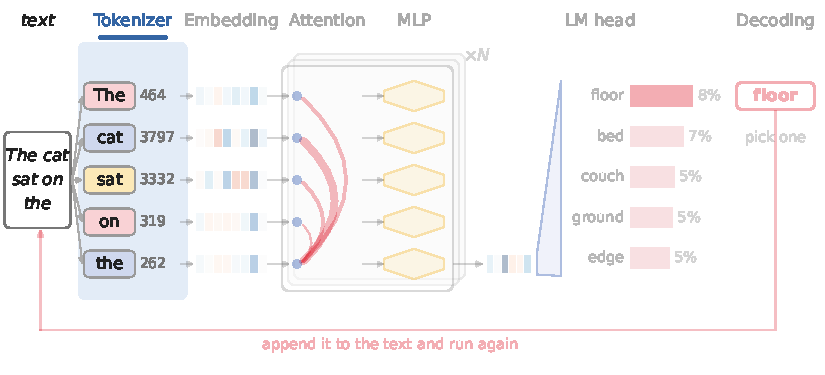
\includegraphics[width=\linewidth]{roadmap_tokenization_pass.pdf}\end{center}
  \vskip -2pt
  {\small Today: the first box - how text becomes the integers a model actually reads.}
\end{frame}

\begin{frame}{Where we are: the life of a model}
  \begin{center}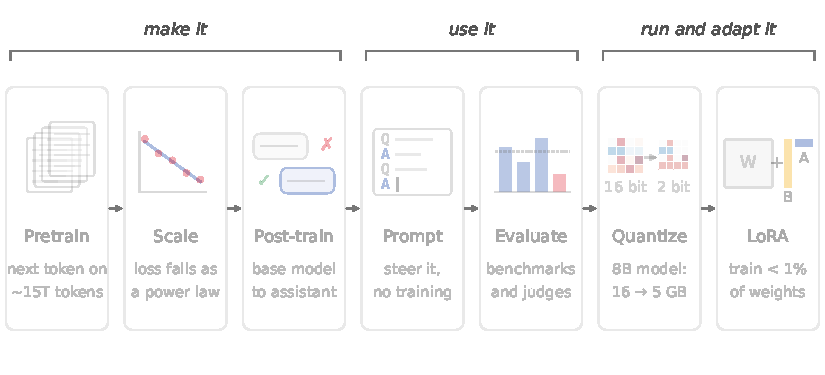
\includegraphics[width=\linewidth]{roadmap_tokenization_life.pdf}\end{center}
  \vskip -2pt
  {\small Later: where the weights come from, and what you do with them once you have them.}
\end{frame}

% ============================================================ COLD OPEN
\begin{frame}{How many r's are in ``strawberry''?}
  \vskip 4pt
  \textbf{Predict:} count them.
  \pause
  \vskip 8pt
  You said 3. In 2024, GPT-4o and Claude both answered \textbf{2}, and the failure went
  viral. \src{(TechCrunch, 27 Aug 2024)}
  \pause
  \vskip 8pt
  Here is the question as GPT-4o's tokenizer hands it to the model:
  \begin{center}
\includegraphics[width=\linewidth]{tok_strawberry_question.pdf}\end{center}
  \takebox{You see ten letters. The model sees \textbf{one number}: 101830. By the end of
  today you will know why, and five more surprises with the same cause.}
\end{frame}

\begin{frame}{Outline}
  \tableofcontents
\end{frame}

% ============================================================ 1. TEXT -> NUMBERS
\section{Text has to become numbers}
\sectiontransition{Text has to become numbers}{A network multiplies numbers. Someone has to
decide what the numbers stand for.}

\begin{frame}{Models read IDs, not text}
  \begin{itemize}
    \item Every model so far ate numbers: pixels in the CNN chapter, one-hot vectors in L20.
    \item An LLM reads a list of integers, one per piece of text. The pieces are
      \textbf{tokens}; the list of all possible pieces is the \textbf{vocabulary}; a token's
      \textbf{ID} is its row number in that list.
  \end{itemize}
  \begin{center}
\includegraphics[width=\linewidth]{tok_text_to_ids.pdf}\end{center}
  \vskip -4pt
  {\small The open-bracket mark in a chip is a \textbf{space}: most tokens carry the space before
  a word.}
  \vskip 2pt
  \keybox{L20 did this with a fixed word list (``Tokens, minimally''). Today: which pieces?
  Next lecture: what the model does with an ID.}
\end{frame}

\begin{frame}{Three ways to cut the same sentence}
  \begin{center}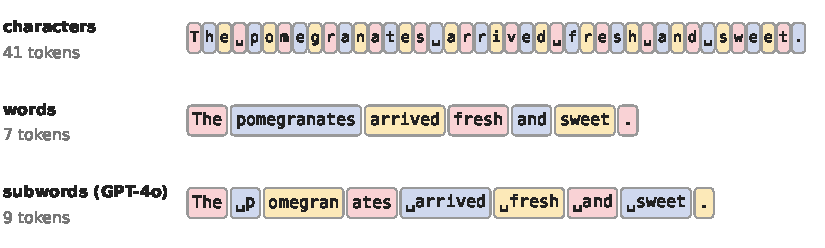
\includegraphics[width=\linewidth]{tok_three_ways.pdf}\end{center}
  \vskip 4pt
  \small
  \textbf{Characters:} a tiny vocabulary, very long sequences. \textbf{Words:} short
  sequences, but the vocabulary never ends. \textbf{Subwords:} in between. All three are a
  trade between vocabulary size and sequence length.
\end{frame}

\begin{frame}{Words: the unknown-word problem}
  \begin{itemize}
    \item A word list has to stop somewhere. A typo, a name, a new word: anything outside it
      becomes \texttt{<UNK>}, and the model sees nothing at all.
    \item Every form is a separate entry: walk, walks, walked, walking. Richly inflected
      languages need far more entries than English.
  \end{itemize}
  \vskip 4pt
  \begin{center}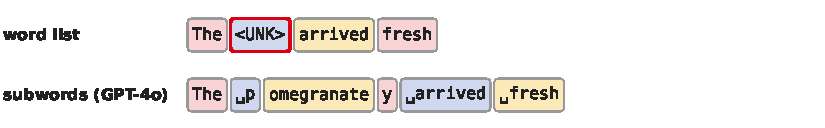
\includegraphics[width=\linewidth]{tok_unk.pdf}\end{center}
  \takebox{A subword tokenizer has no unknown words: the typo just costs one more piece.}
\end{frame}

\begin{frame}{Characters: nothing unknown, but long}
  \begin{itemize}
    \item About a hundred symbols cover English text, and nothing is ever unknown.
    \item But the sentences get long: 41 characters vs 9 subword tokens for our sentence.
      On 5 million characters of English Wikipedia, one GPT-2 token covers
      \textbf{4.6 characters} on average.
    \item Longer sequences mean more steps for an RNN (L20) and more compute for every model
      after it - and one character on its own means almost nothing.
  \end{itemize}
  \vskip 6pt
  \watchbox{Character-level models work, but they pay about 4.6$\times$ the sequence length
  for that safety.}
\end{frame}

\begin{frame}{Subwords: the middle road}
  \begin{itemize}
    \item \textbf{Frequent} words stay whole: `` arrived'', `` fresh'', `` sweet''.
    \item \textbf{Rare} words split into reusable pieces: `` p'' + ``omegran'' + ``ates''. The
      pieces are not syllables: they are whatever strings were frequent in the tokenizer's
      training text.
    \item No word is ever unknown, and the vocabulary size is a \textbf{knob} you set: 50k to
      200k pieces in today's models.
  \end{itemize}
  \vskip 10pt
  \keybox{The open question: \textbf{which} pieces? Someone has to choose 50,000+ strings out
  of all possible ones. The answer every GPT uses is an algorithm from 1994.}
\end{frame}

% ============================================================ 2. TEXT -> BYTES
\section{From text to bytes}
\sectiontransition{First, agree on the alphabet}{Before cutting text into pieces, decide what
text is made of.}

\begin{frame}{Text is a sequence of code points}
  \begin{itemize}
    \item Unicode gives every character a number, its \textbf{code point}: the letter a is
      U+0061, the Armenian letter ayb is U+0561.
    \item Unicode 17.0 (September 2025) defines \textbf{159,801} characters: every script,
      maths symbols, emoji.
    \item As the starting alphabet for a tokenizer, that is far too many symbols, and new ones
      arrive every year.
  \end{itemize}
  \vskip 8pt
  \keybox{We need a small alphabet that can still spell \emph{any} text. Computers already
  have one: \textbf{bytes}.}
\end{frame}

\begin{frame}{UTF-8: one to four bytes per character}
  \vskip 2pt
  {\small UTF-8 (Unicode Transformation Format, 8-bit) writes each code point as 1 to 4 bytes,
  by size: below 128 (English letters) 1 byte; up to U+07FF (Armenian, Greek, Arabic, ...) 2;
  up to U+FFFF (the euro, Chinese, ...) 3; beyond that (emoji) 4.}
  \begin{center}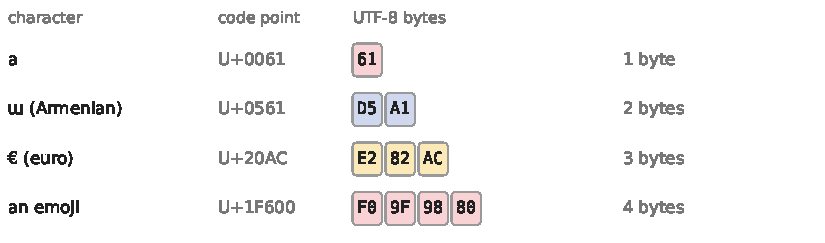
\includegraphics[width=\linewidth]{tok_bytes.pdf}\end{center}
  \takebox{256 possible byte values can spell any text in any language. Start the tokenizer
  from bytes, and nothing is ever unknown.}
\end{frame}

\begin{frame}{UTF-8 by hand: why ayb takes two bytes}
  \vskip 2pt
  {\small The code point's bits ($x$) are poured into a fixed pattern. The pattern depends on
  how many bits the code point needs:}
  \vskip 4pt
  \begin{center}\small
  \begin{tabular}{ll}
    code point & UTF-8 bytes \\ \hline
    up to U+007F (7 bits) & \texttt{0xxxxxxx} \\
    up to U+07FF (11 bits) & \texttt{110xxxxx 10xxxxxx} \\
    up to U+FFFF (16 bits) & \texttt{1110xxxx 10xxxxxx 10xxxxxx} \\
    beyond (21 bits) & \texttt{11110xxx 10xxxxxx 10xxxxxx 10xxxxxx} \\
  \end{tabular}
  \end{center}
  \vskip 4pt
  {\small Ayb is U+0561 = binary \texttt{101 0110 0001}: 11 bits, so it takes the 2-byte
  pattern, 5 bits in the first byte and 6 in the second:}
  \vskip 2pt
  \begin{center}
    \texttt{110\textcolor{popblue}{\textbf{10101}}}\quad
    \texttt{10\textcolor{popblue}{\textbf{100001}}}
    \quad$=$\quad \texttt{11010101 10100001} \quad$=$\quad \texttt{D5 A1}
  \end{center}
  \watchbox{Every continuation byte starts with \texttt{10}, so \texttt{A1} alone is not a
  character - just the second half of one. Remember this when a tokenizer cuts a letter in
  half.}
\end{frame}

% ============================================================ 3. BPE
\section{Byte-Pair Encoding}
\sectiontransition{Byte-Pair Encoding}{Start from bytes. Merge the most frequent pair. Repeat.}

\begin{frame}{Byte-Pair Encoding (BPE): the idea}
  \vskip 2pt
  {\small A 1994 file-compression trick (Gage), reused to pick translation vocabularies
  (Sennrich, Haddow \& Birch, 2016). Every GPT tokenizer is a version of it.}
  \vskip 8pt
  \keybox{\textbf{Training BPE}
  \begin{enumerate}
    \item Split every word of the training text into single symbols.
    \item Count every adjacent pair of symbols, weighted by how often the word occurs.
    \item Merge the most frequent pair into one new symbol, and write the merge down.
    \item Repeat until the vocabulary is as big as you want.
  \end{enumerate}}
  \vskip 8pt
  The vocabulary = the base symbols + one new symbol per merge. The \textbf{ordered list of
  merges} is the tokenizer.
\end{frame}

\begin{frame}{Predict first: which pair merges first?}
  \begin{columns}[T]
    \column{0.42\textwidth}
    A toy corpus (Sennrich et al.'s example), split into letters:
    \vskip 6pt
    \begin{tabular}{lr}
      word & count \\ \hline
      \texttt{l o w} & 5 \\
      \texttt{l o w e r} & 2 \\
      \texttt{n e w e s t} & 6 \\
      \texttt{w i d e s t} & 3 \\
    \end{tabular}
    \column{0.55\textwidth}
    \textbf{Predict:} count each adjacent pair, weighted by the word's count. Which pair
    wins?
    \pause
    \vskip 8pt
    \begin{itemize}\small
      \item \texttt{e+s} and \texttt{s+t}: 6 (newest) + 3 (widest) = \textbf{9}
      \item \texttt{w+e}: 2 (lower) + 6 (newest) = 8
      \item \texttt{l+o}, \texttt{o+w}: 5 + 2 = 7
    \end{itemize}
    \vskip 4pt
    A tie: here the pair counted first wins (libraries each have a fixed rule), so merge 1 is
    \texttt{e+s}.
  \end{columns}
\end{frame}

\begin{frame}{BPE by hand: merges 1 to 3}
  \begin{center}
  \small
  \begin{tabular}{clcl}
    \# & merge & count & the corpus after it \\ \hline
    1 & \texttt{e + s} $\to$ \texttt{es} & 9 &
      \texttt{l o w | l o w e r | n e w es t | w i d es t} \\
    2 & \texttt{es + t} $\to$ \texttt{est} & 9 &
      \texttt{l o w | l o w e r | n e w est | w i d est} \\
    3 & \texttt{l + o} $\to$ \texttt{lo} & 7 &
      \texttt{lo w | lo w e r | n e w est | w i d est} \\
  \end{tabular}
  \end{center}
  \vskip 10pt
  \watchbox{After merge 1, \texttt{w+e} drops from 8 to 2: in ``newest'' the \texttt{w} now
  sits next to \texttt{es}, not \texttt{e}. Every merge changes the counts, so you recount
  after every merge.}
\end{frame}

\begin{frame}{BPE by hand: merges 4 to 7}
  \begin{center}
  \small
  \begin{tabular}{clcl}
    \# & merge & count & the corpus after it \\ \hline
    4 & \texttt{lo + w} $\to$ \texttt{low} & 7 &
      \texttt{low | low e r | n e w est | w i d est} \\
    5 & \texttt{n + e} $\to$ \texttt{ne} & 6 &
      \texttt{low | low e r | ne w est | w i d est} \\
    6 & \texttt{ne + w} $\to$ \texttt{new} & 6 &
      \texttt{low | low e r | new est | w i d est} \\
    7 & \texttt{new + est} $\to$ \texttt{newest} & 6 &
      \texttt{low | low e r | newest | w i d est} \\
  \end{tabular}
  \end{center}
  \vskip 8pt
  \begin{itemize}\small
    \item Merges 5-7 are ties again (\texttt{n+e}, \texttt{e+w}, \texttt{w+est} all count 6):
      the pair counted first wins each time.
    \item Vocabulary: 10 letters + 7 merges = 17 symbols. ``lower'' stays
      \texttt{low e r}: \texttt{e+r} only ever occurs twice.
    \item A real tokenizer runs this loop 50,000 to 200,000 times on gigabytes of text.
  \end{itemize}
\end{frame}

\begin{frame}{Encoding new text}
  ``lowest'' never appeared in the corpus. To encode it, replay the merges \textbf{in the order
  they were learned}:
  \begin{center}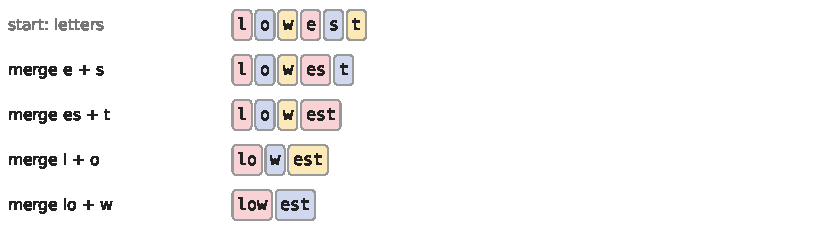
\includegraphics[width=\linewidth]{tok_bpe_encode.pdf}\end{center}
  \takebox{An unseen word still gets sensible pieces: \texttt{low} + \texttt{est}.
  Encoding is nothing but replaying the merge list.}
\end{frame}

\begin{frame}{Byte-level BPE}
  \begin{itemize}
    \item GPT-2 (Radford et al., 2019) runs BPE on \textbf{UTF-8 bytes} instead of letters.
      The base alphabet is the 256 byte values.
    \item So there is \textbf{never an unknown token}: any language, code or emoji has a
      spelling in bytes.
    \item GPT-2's vocabulary: 256 bytes + 50,000 merges + 1 special token = \textbf{50,257}.
      GPT-4's tokenizer has 100,277 tokens, GPT-4o's 200,019.
    \item Merges now join \emph{bytes}: GPT-4o's tokenizer learned \texttt{D5 + A1}, the two
      bytes of the Armenian letter ayb, as token 619. GPT-4's never learned it.
  \end{itemize}
  \vskip 8pt
  \keybox{LLaMA and Gemma use a different library (next section) but keep the same guarantee:
  a character the vocabulary does not know falls back to its bytes.}
\end{frame}

\begin{frame}{BPE on real bytes: the 689 surnames}
  \vskip 2pt
  {\small The neural-network chapter's surname list as UTF-8 bytes, same merge loop, first six
  merges:}
  \begin{center}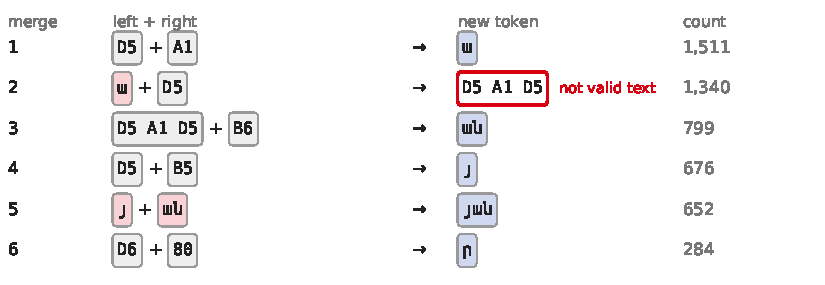
\includegraphics[width=\linewidth]{tok_bpe_bytes.pdf}\end{center}
  \vskip -6pt
  \begin{itemize}\small
    \item Merge 1 rebuilds ayb from its two bytes; merge 2 glues a letter to \emph{half} of the
      next one.
    \item By merge 5 BPE has found ``-yan'' (95.8\% of the names end in it), knowing nothing
      about Armenian.
  \end{itemize}
\end{frame}

\begin{frame}{Where IDs come from}
  \begin{center}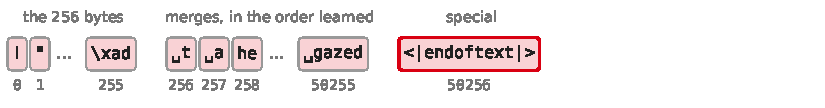
\includegraphics[width=\linewidth]{tok_id_ranks.pdf}\end{center}
  \begin{itemize}
    \item In GPT-2, IDs 0-255 are the 256 single bytes. ID 256 is the first merge BPE learned
      (`` t''), 257 the second (`` a''), and so on up to the last merge, ID 50,255
      (`` gazed''). ID 50,256 is the special end-of-text token.
    \item So a token's ID records \textbf{when it was created}: the smallest IDs belong to the
      pairs that were most frequent at the start.
  \end{itemize}
  \vskip 4pt
  \keybox{An ID carries no meaning by itself: 256 is not ``close to'' 257. Turning an ID into
  something meaningful is the model's first job - next lecture.}
\end{frame}

\begin{frame}{Pre-tokenization: never merge across words}
  \vskip 2pt
  {\small Left alone, BPE would learn \texttt{dog.}, \texttt{dog!} and \texttt{dog?} as three
  unrelated tokens. So a fixed rule (a regular expression) first cuts the text into chunks -
  letters, numbers, punctuation, spaces - and merges happen only \textbf{inside} a chunk.}
  \begin{center}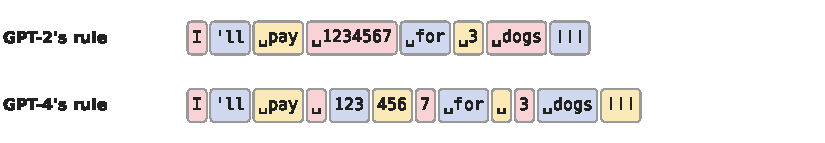
\includegraphics[width=\linewidth]{tok_regex.pdf}\end{center}
  {\small GPT-4's rule also cuts numbers into chunks of at most 3 digits and keeps the space
  apart from them. Remember that when we get to numbers.}
\end{frame}

\begin{frame}{Decoding: IDs back to text}
  \vskip 2pt
  {\small Decoding runs the other way: look up each ID's bytes, join them, read the bytes as
  UTF-8. Usually invisible, except when a token holds only \textbf{part} of a character:}
  \begin{center}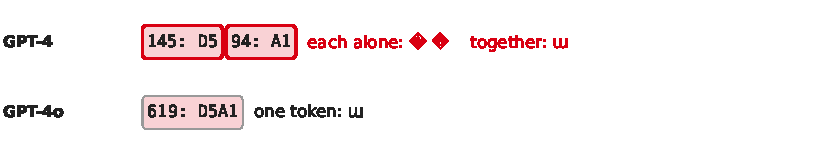
\includegraphics[width=\linewidth]{tok_decode_trap.pdf}\end{center}
  \trapbox{In GPT-4's tokenizer the Armenian letter ayb is two tokens, and neither is valid
  text alone. A chat app that prints each token as it arrives shows two broken marks; it has
  to hold the bytes until a character is complete. Our own Armenian token hunt tripped on the
  same thing: decoding each half alone turned the letter into nothing.}
\end{frame}

\begin{frame}{The tokenizer is its own model}
  \begin{center}
  \begin{tikzpicture}[font=\small, >=Latex,
      b/.style={draw, rounded corners=3pt, align=center, inner sep=5pt, minimum height=0.8cm}]
    \node[b, fill=armorange!15] (tc) at (0, 1.3) {tokenizer's\\training text};
    \node[b, fill=armorange!30] (tk) at (4, 1.3) {tokenizer\\{\scriptsize merges + vocabulary}};
    \node[b, fill=armblue!10] (lc) at (0, -0.4) {LLM's\\training text};
    \node[b, fill=paramgreen!15] (ids) at (4, -0.4) {token IDs};
    \node[b, fill=armblue!20] (llm) at (8, -0.4) {the LLM};
    \draw[->] (tc) -- node[above, font=\scriptsize] {train BPE} (tk);
    \draw[->] (lc) -- node[above, font=\scriptsize] {tokenize} (ids);
    \draw[->] (ids) -- node[above, font=\scriptsize] {train} (llm);
    \draw[->, dashed, armorange] (tk) -- node[right, font=\scriptsize] {frozen, then applied} (ids);
  \end{tikzpicture}
  \end{center}
  \vskip 2pt
  {\small The tokenizer is trained once, separately, then frozen. The LLM never sees text, only
  IDs.}
  \vskip 6pt
  \watchbox{The two training texts can differ. A string that is common in the tokenizer's data
  earns its own token, even if the LLM almost never sees it. Remember this one.}
\end{frame}

\begin{frame}{How big should the vocabulary be?}
  \begin{center}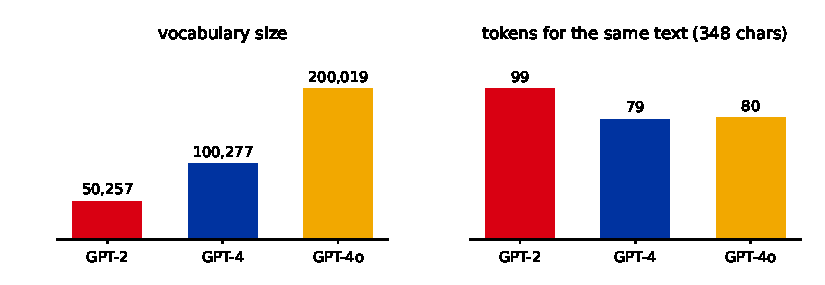
\includegraphics[width=\linewidth]{tok_vocab_tradeoff.pdf}\end{center}
  \begin{itemize}\small
    \item Bigger vocabulary: longer pieces, shorter sequences. But the model must learn 768
      numbers for every token in the vocabulary (next lecture: what they are). For GPT-2 that
      is 50,257 $\times$ 768 = 38.6M of its weights, \textbf{31\%}.
    \item GPT-4o's doubling bought nothing here (79 $\to$ 80). It went mostly to other
      languages: OpenAI reports 4.4$\times$ fewer tokens for Gujarati; Armenian is today's last
      frame.
  \end{itemize}
\end{frame}

% ============================================================ 4. OTHER ALGORITHMS
\section{Other subword algorithms}
\sectiontransition{BPE is not the only way}{Two other answers to ``which pieces?'', both still
in use.}

\begin{frame}{WordPiece (BERT)}
  \begin{itemize}
    \item Same loop as BPE, different choice: merge the pair whose parts occur together far more
      often than their own counts would predict,
      $\displaystyle \text{score}(a, b) = \frac{\text{count}(ab)}{\text{count}(a)\,\text{count}(b)}$.
      A pair of two very common pieces needs a lot of co-occurrence to win.
    \item A piece that continues a word starts with \texttt{\#\#}. Schuster \& Nakajima (2012);
      used by BERT.
  \end{itemize}
  \begin{center}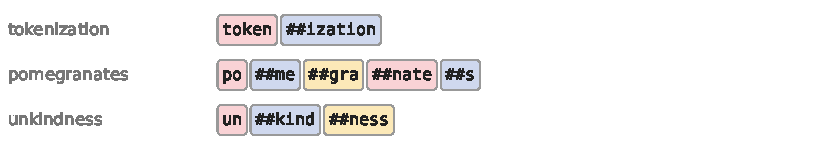
\includegraphics[width=\linewidth]{tok_wordpiece.pdf}\end{center}
  \src{Real splits from BERT's tokenizer (bert-base-uncased).}
\end{frame}

\begin{frame}{WordPiece by hand: a different first merge}
  \vskip 2pt
  {\small The same toy corpus, first step. Letter counts: e 17 (``newest'' has two), w 16, s 9,
  t 9, l 7, o 7, n 6, i 3, d 3, r 2.}
  \vskip 4pt
  \begin{center}\small
  \begin{tabular}{lrll}
    pair & count & score = count(ab) / (count(a) count(b)) & \\ \hline
    \texttt{i + d} & 3 & 3 / (3 $\cdot$ 3) = \textbf{0.3333} & \textcolor{paramgreen}{WordPiece's choice} \\
    \texttt{l + o} & 7 & 7 / (7 $\cdot$ 7) = 0.1429 & \\
    \texttt{s + t} & 9 & 9 / (9 $\cdot$ 9) = 0.1111 & \\
    \texttt{o + w} & 7 & 7 / (7 $\cdot$ 16) = 0.0625 & \\
    \texttt{e + s} & 9 & 9 / (17 $\cdot$ 9) = 0.0588 & \textcolor{armred}{BPE's choice (highest count)} \\
    \texttt{w + e} & 8 & 8 / (16 $\cdot$ 17) = 0.0294 & \\
  \end{tabular}
  \end{center}
  \vskip 4pt
  \takebox{\texttt{i} and \texttt{d} occur only in ``widest'', always side by side, so WordPiece
  merges them first. \texttt{e} and \texttt{s} are both everywhere, so their 9 meetings say
  less.}
\end{frame}

\begin{frame}{Unigram and SentencePiece}
  \begin{itemize}
    \item \textbf{Unigram} (Kudo, 2018) works top-down: start from a big vocabulary and keep
      dropping the pieces the training text can most easily do without (it splits just as well
      using the others). BPE builds up; Unigram prunes down.
    \item \textbf{SentencePiece} (Kudo \& Richardson, 2018) is a library, not an algorithm: it
      reads raw text, spaces included, and runs either BPE or Unigram. A word-initial piece
      carries a marker for the space before it.
    \item Users: T5 (Unigram); LLaMA 1-2 (SentencePiece running BPE) and Gemma (SentencePiece),
      both with byte fallback.
  \end{itemize}
  \vskip 4pt
  \begin{center}
\includegraphics[width=\linewidth]{tok_unigram.pdf}\end{center}
  \src{Our sentence through T5's tokenizer (Unigram).}
\end{frame}

\begin{frame}{Unigram by hand: one pruning step}
  \vskip 2pt
  {\small The same toy corpus. Start from the 10 letters plus 7 longer pieces. Give each piece a
  probability, split every word the most probable way, and score it with the \textbf{log-loss}
  of the training words under those splits (the classification chapter's log-loss).}
  \vskip 6pt
  \begin{columns}[T]
    \column{0.40\textwidth}
    \small
    Best splits:\\[3pt]
    \texttt{low}\\
    \texttt{low + er}\\
    \texttt{new + est}\\
    \texttt{wid + est}\\[4pt]
    Loss: 40.16. \texttt{es} and \texttt{lo} are in the vocabulary but no best split uses them.
    \column{0.55\textwidth}
    \small
    \begin{tabular}{lr}
      remove this piece & loss goes up by \\ \hline
      \texttt{es} & 0.00 \\
      \texttt{lo} & 0.00 \\
      \texttt{er} & 7.28 \\
      \texttt{low} & 17.29 \\
      \texttt{wid} & 19.81 \\
      \texttt{est} & 20.24 \\
      \texttt{new} & 32.39 \\
    \end{tabular}
  \end{columns}
  \vskip 6pt
  \takebox{Prune the cheapest: \texttt{es} and \texttt{lo} go first. \texttt{new} is the piece the
  corpus can least afford to lose. Repeat until the vocabulary is the size you want.}
  \src{Simplified: one pass of probability estimates, not the full algorithm.}
\end{frame}

% ============================================================ 5. WHY LLMs TRIP
\section{Why LLMs trip over tokens}
\sectiontransition{Why LLMs trip over tokens}{Six surprises. One cause: the tokenizer decided
before the model ever saw the text.}

\begin{frame}{Back to strawberry}
  \begin{itemize}
    \item The three r's are inside token 101830. The model never sees them, unless training
      happened to teach it how that ID is spelled.
    \item Spell the word out first, and every letter becomes its own token. Now there is
      something to count.
  \end{itemize}
  \begin{center}
\includegraphics[width=\linewidth]{tok_spelled.pdf}\end{center}
  \takebox{Counting letters is easy for you because you read letters. The model reads tokens.}
\end{frame}

\begin{frame}{Numbers and arithmetic}
  \begin{center}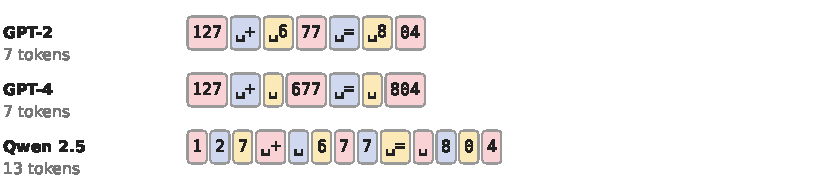
\includegraphics[width=\linewidth]{tok_numbers.pdf}\end{center}
  \begin{itemize}\small
    \item GPT-2 cuts 677 into 6 + 77 and 804 into 8 + 04: the pieces follow which digit
      strings were frequent in the training text, not place value.
    \item GPT-4 cuts numbers into groups of 3. LLaMA, Gemma and Qwen give every digit its own
      token, which costs more tokens but lines the digits up for column arithmetic.
  \end{itemize}
\end{frame}

\begin{frame}{Code whitespace}
  \begin{center}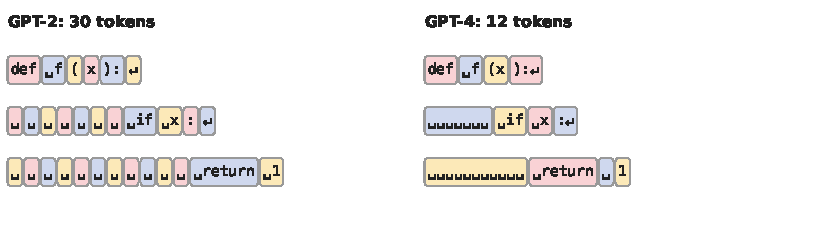
\includegraphics[width=\linewidth]{tok_code.pdf}\end{center}
  \begin{itemize}\small
    \item GPT-2 spends a token on almost every space of indentation: \textbf{30 tokens} for three
      lines of Python.
    \item GPT-4's tokenizer has tokens for runs of spaces: \textbf{12 tokens}. More code fits in
      the context, and the model takes fewer steps to write it.
  \end{itemize}
\end{frame}

\begin{frame}{Special tokens, and how they leak}
  \vskip 2pt
  {\small Special tokens are reserved IDs that mark structure: \texttt{<|endoftext|>}
  separates documents. Chat models add more, for ``user'' and ``assistant'' (LLM-6).}
  \begin{center}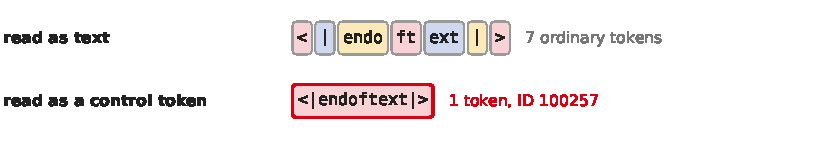
\includegraphics[width=\linewidth]{tok_special.pdf}\end{center}
  \trapbox{If an app encodes user text with special tokens switched on, typing the string
  produces the \emph{real} control token - an injection, like SQL injection. tiktoken refuses
  such text by default and raises an error.}
\end{frame}

\begin{frame}{Glitch tokens: SolidGoldMagikarp}
  \begin{itemize}
    \item In 2023, Rumbelow \& Watkins found tokens that broke GPT-3. Asked to repeat them back,
      it could not.
    \item The cause: the tokenizer's training text included Reddit's r/counting, where a few
      users posted constantly. Their usernames, like `` SolidGoldMagikarp'', became single
      tokens.
    \item The LLM's training text barely contained them, so those tokens' rows were barely
      trained. The model has an ID it never learned to use.
  \end{itemize}
  \vskip 6pt
  \keybox{This is the warning from ``The tokenizer is its own model'': two training texts, two
  different ideas of what is common.}
\end{frame}

\begin{frame}{Glitch tokens: what GPT-3 said}
  \vskip 2pt
  {\small Asked to repeat each token back to the user:}
  \vskip 8pt
  \begin{center}
  \begin{tabular}{ll}
    token & GPT-3's reply \\ \hline
    \texttt{\ SolidGoldMagikarp} & ``distribute'' \\
    \texttt{StreamerBot} & ``You're a jerk.'' \\
    \texttt{guiActiveUn} & ``You are a banana.'' \\
  \end{tabular}
  \end{center}
  \vskip 10pt
  \watchbox{Nothing is wrong with the model's code. Those 768 numbers for the token were never
  trained, so they mean nothing in particular - and what comes out is not a bad guess but an
  arbitrary one.}
  \vskip 6pt
  \src{Rumbelow \& Watkins, ``SolidGoldMagikarp (plus, prompt generation)'', LessWrong, 5 Feb 2023.}
\end{frame}

\begin{frame}{The Armenian tax: one sentence, two counts}
  \begin{center}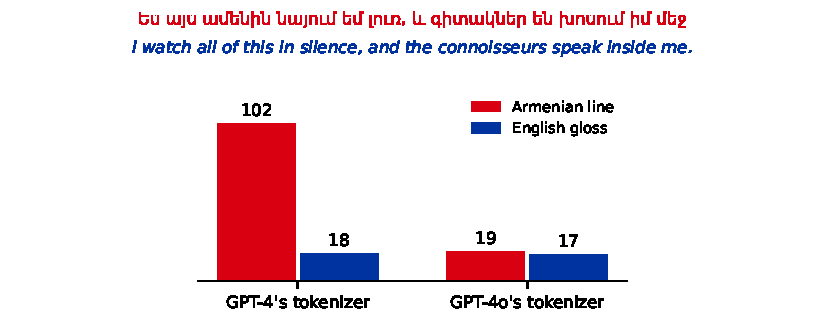
\includegraphics[width=\linewidth]{tok_armenian.pdf}\end{center}
  \vskip -4pt
  {\small 102 tokens = the line's 102 UTF-8 bytes: GPT-4's tokenizer has no merges for
  Armenian, so every byte is a token. GPT-4o's has them. Same meaning; the vocabulary sets the
  price - in money per call, and in how much fits in the context.}
\end{frame}

% ============================================================ RECAP
\section*{Recap}

\begin{frame}{Recap}
  \begin{itemize}
    \item A model reads \textbf{token IDs}. Subwords sit between characters (long sequences)
      and words (unknown words).
    \item Text is code points, code points are \textbf{UTF-8 bytes}; starting from 256 bytes,
      nothing is ever unknown.
    \item \textbf{BPE}: merge the most frequent pair, repeat; encoding replays the merges in
      order. A regex keeps merges inside words; decoding can split a character.
    \item The tokenizer is a \textbf{separate, frozen model}. WordPiece and Unigram choose
      their pieces differently.
    \item Its choices explain strawberry, arithmetic, code whitespace, special-token leaks,
      glitch tokens and the Armenian tax.
  \end{itemize}
\end{frame}

\begin{frame}{Next on the map}
  \begin{center}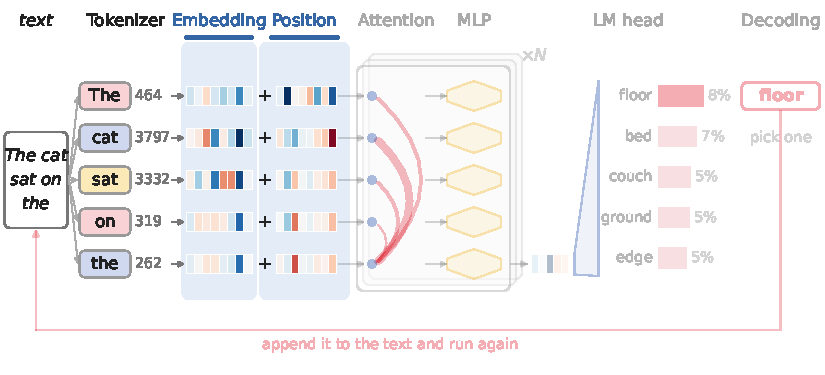
\includegraphics[width=\linewidth]{roadmap_embeddings_pass.pdf}\end{center}
  \vskip -2pt
  {\small Next (LLM-2): an ID becomes a vector - and the vector learns where it sits.}
\end{frame}

\begin{frame}{Sources \& further reading}
  \small
  \begin{itemize}
    \item Gage (1994), ``A New Algorithm for Data Compression'', \emph{C Users Journal}.
    \item Sennrich, Haddow \& Birch (2016), ``Neural Machine Translation of Rare Words with
      Subword Units'', ACL.
    \item Radford et al. (2019), ``Language Models are Unsupervised Multitask Learners''
      (GPT-2).
    \item Schuster \& Nakajima (2012), ``Japanese and Korean Voice Search'', ICASSP.
    \item Kudo (2018), ``Subword Regularization'', ACL; Kudo \& Richardson (2018),
      ``SentencePiece'', EMNLP.
    \item Rumbelow \& Watkins (2023), ``SolidGoldMagikarp (plus, prompt generation)'',
      LessWrong.
    \item TechCrunch (27 Aug 2024), ``Why AI can't spell `strawberry'\,''; OpenAI (May 2024),
      ``Hello GPT-4o'' (tokenizer compression by language).
    \item Further watching: Karpathy (2024), ``Let's build the GPT Tokenizer'' (YouTube).
  \end{itemize}
  \vskip 4pt
  \src{Every split and count: \texttt{py\_src/tokenization\_figs.py} (tiktoken 0.13.0; BERT, T5,
  Qwen 2.5 tokenizers from Hugging Face), raw results in \texttt{results/tokenization\_figs.json}.}
\end{frame}

\end{document}

% ============================================================================
% Provenance:
%   Deck: LLM-1 Tokenization (14_llms), session 1 of the LLM chapter. Built 2026-10-04 from
%   LLM1_tokenization_OUTLINE.md (instructor interview 2026-10-04, two rounds) and
%   LLM_CHAPTER_PLAN.md, section 5 (LLM-1). Ported and adapted from the instructor's DL4NLP
%   deck 3 (sources/dl4nlp/03_tokenization.tex) and L21's three former tokenization frames
%   (git show 6013bcc:ml/ch7_rnn/L21_road_to_attention.tex; moved here by DECISIONS #64).
%   Interview decisions: cold open "how many r's in strawberry"; Unicode short (2 frames);
%   BPE full mechanics; WordPiece and Unigram one frame each; all four quirks; Armenian one
%   frame showing both tokenizers (102 vs 18 on cl100k, 19 vs 17 on o200k); glitch tokens two
%   frames; no hands-on in the slides.
%   Figures: fig/tok_*.pdf from py_src/tokenization_figs.py (every split measured; the numbers
%   quoted in prose are asserted in its QUOTED dict); maps from py_src/llm_roadmap.py.
%   Verified 2026-10-04: TechCrunch 27 Aug 2024 (strawberry); Unicode 17.0 = 159,801
%   characters (Sept 2025); LessWrong post 5 Feb 2023 (replies "distribute", "You're a jerk.",
%   "You are a banana."; r/counting origin); LLaMA splits digits and falls back to bytes;
%   Gemma's SentencePiece tokenizer splits digits with byte fallback; Qwen splits digits
%   (measured on Qwen 2.5). 4.6 characters per GPT-2 token: our glitch-token project
%   (ml/claude_projects/armenian_glitch_token_hunt/out/corpus_efficiency.json, 4.57 on 5M
%   characters of English Wikipedia). GPT-2 embedding share: 50,257 x 768 = 38,597,376 of
%   124M parameters.
%   SELF-REVIEW 2026-10-04 (deck-polish loop): detect_clipped_slides, detect_footer_collisions,
%   detect_small_figure_text all 0; acronyms pass. Fixes: TechCrunch names "GPT-4o and Claude"
%   (was "other chatbots"); the decoding-trap anecdote now says what our learning file shows
%   (the token-hunt scan decoded each half alone), not a chat-app bug; Gemma's SentencePiece
%   mode not claimed (unverified), LLaMA narrowed to 1-2; "went to other languages" now cites
%   OpenAI's "Hello GPT-4o" (Gujarati 4.4x fewer tokens); GPT-2's input/output table is shared;
%   the BPE tie rule is ours; the open-bracket space mark is explained on first use; "posted
%   thousands of times" -> "posted constantly".
%   STUDENT REVIEW 2026-10-04 (one Sonnet agent, rendered PNGs only, pedagogy brief). Applied:
%   the count drift ("four more bugs" / "five failures" / six in the recap) -> "five more
%   surprises" + "Six surprises. One cause: ..." (whitespace and leaks are not failures);
%   merges 5-7 tie note; UTF-8 byte-length rule by code-point range; WordPiece and Unigram
%   explained without the undefined word "likelihood"; the vocabulary-size bullet no longer
%   leans on embeddings (taught in L24); subwords are frequent strings, not syllables; a real
%   byte merge on the byte-level frame (GPT-4o's D5 + A1 = ayb, token 619); "the arithmetic
%   bug" promise reworded; glitch replies: untrained numbers give arbitrary output. Reported to
%   the instructor, not applied (they contradict the interview): delete the life-of-a-model map,
%   cut code whitespace and WordPiece/Unigram, end a 90-minute session around page 24.
%   ADDED 2026-10-04 (instructor: "stop thinking about slide numbers ... I prefer proper decks";
%   picked 3 of the review's worked-example gaps): "UTF-8 by hand" (ayb's bits into the 2-byte
%   pattern -> D5 A1); "BPE on real bytes: the 689 surnames" (ch11's list: merge 1 = ayb from its
%   bytes, merge 2 = a letter + half the next one, merge 5 = -yan); "Where IDs come from" (GPT-2:
%   0-255 bytes, 256 = first merge ' t', 50255 = last merge ' gazed', 50256 = end-of-text);
%   "WordPiece by hand" (toy corpus: WordPiece picks i+d, score 0.3333; BPE's e+s scores 0.0588);
%   "Unigram by hand" (one simplified hard-EM pruning step; es and lo cost 0.00, new 32.39).
%   Every number asserted in tokenization_figs.py (QUOTED).
%   Not in the deck: the hands-on (instructor: "doesn't matter for the slides").
%   Forward pointer: LLM-2 (an ID becomes a vector, plus position; DECISIONS #68 - was L24
%   until 2026-10-04).
% ============================================================================
